% !TeX root = ../main.tex
% Add the above to each chapter to make compiling the PDF easier in some editors.

%\chapter{PASCAL VOC Void Pixel}


\begin{figure}
	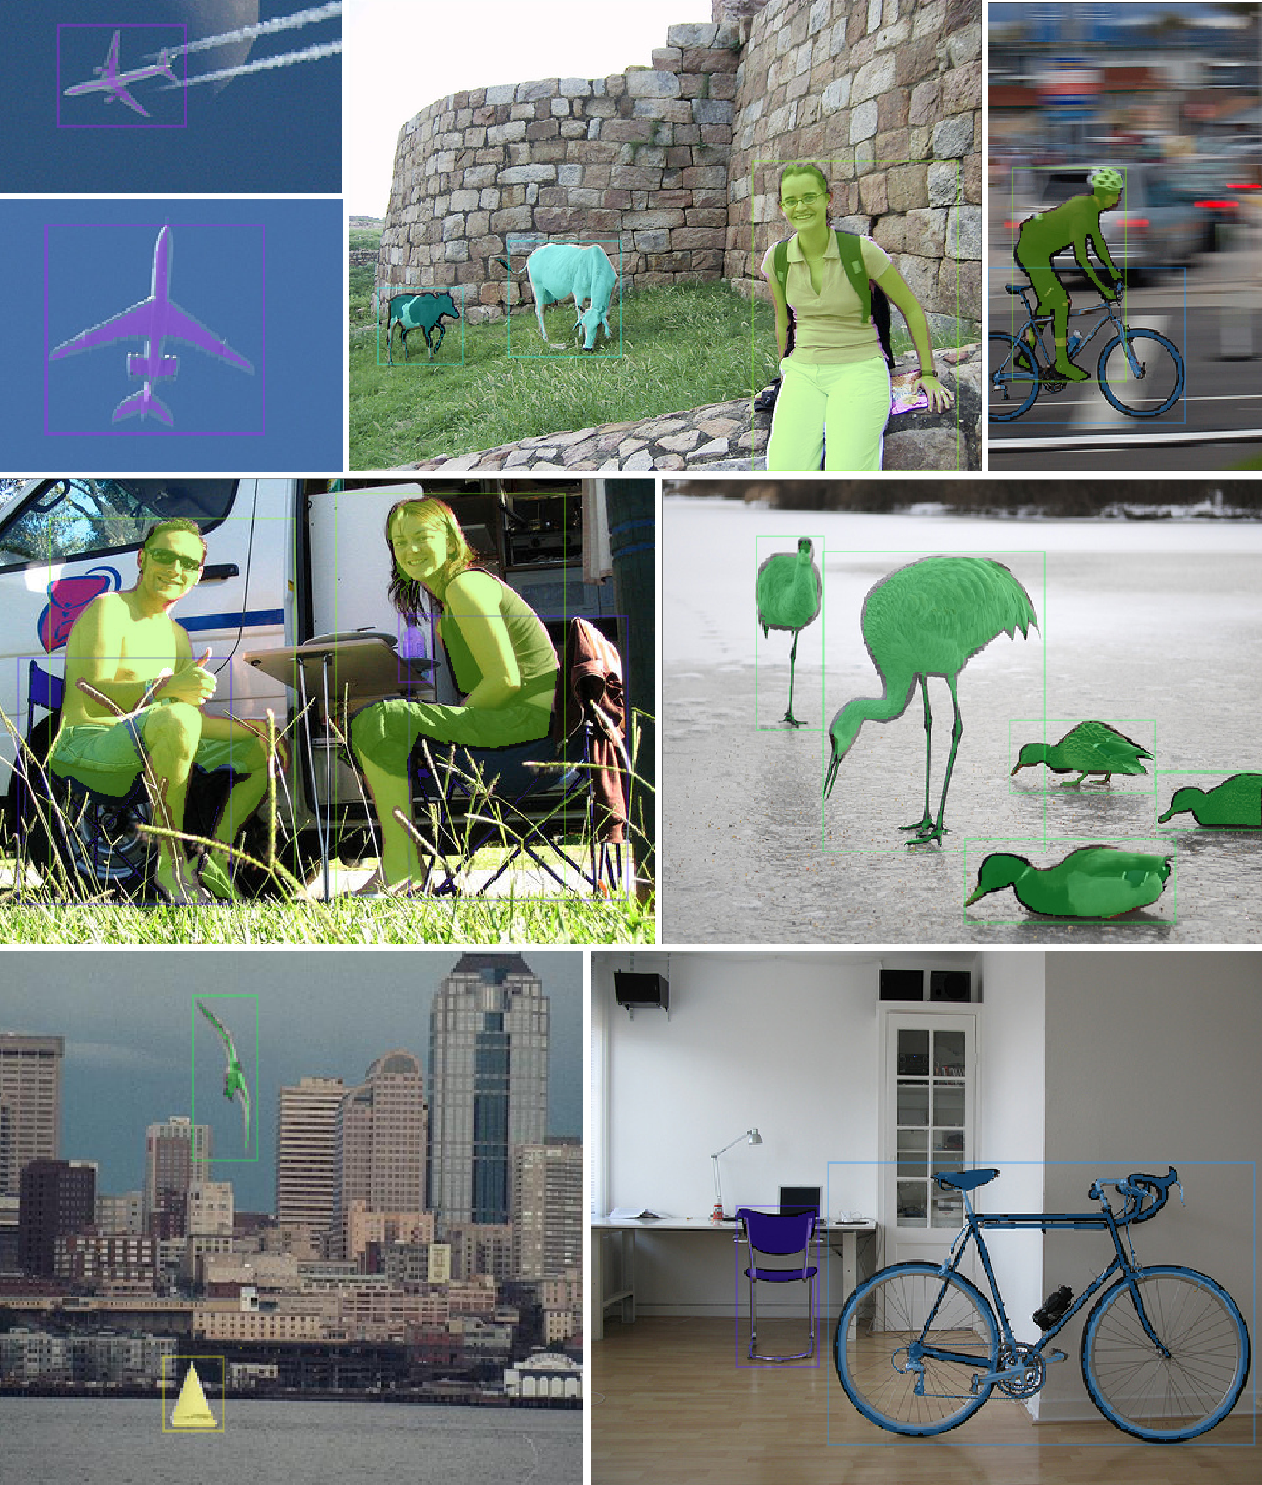
\includegraphics[width=\linewidth]{figures/appendix/pascal_voc/pascal_voc_collage.png}
	\caption[PASCAL VOC images with instance masks]{		
		Images from the PASCAL \gls{voc} dataset \cite{Eve20-PascalVOC}. 
		The object masks are visualized without the \gls{vp}, while the direct edges of the objects are not part of the masks, because they belong to the \gls{vp}.
	 	It can be seen that this \gls{gt} is especially questionable for detailed and overlapping objects.
	}
	\label{fig:appendix_pascal_voc}
\end{figure}